    {\large 電気回路 - 交流・共振 -}

    \begin{multicols}{3}
        \begin{itembox}[l]{交流の概念}
            \begin{figure}[H]
                \label{fig:ac}
                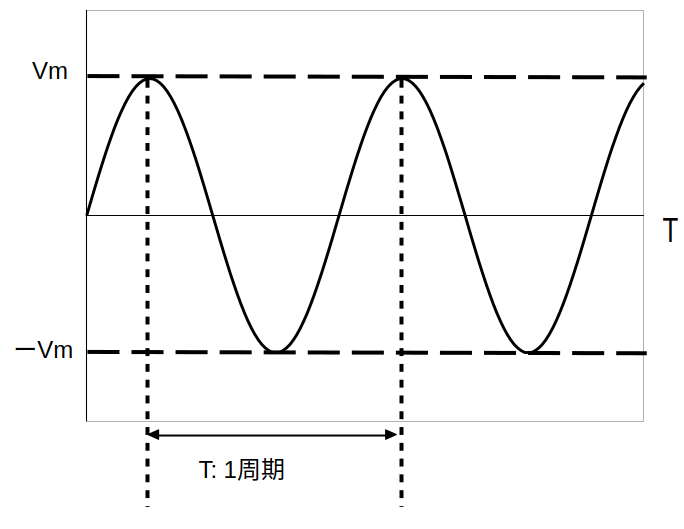
\includegraphics[width=0.9\linewidth]{fig/交流概念.png}
                \caption{交流の波形}
            \end{figure}
            \begin{itemize}
                \item 電流や電圧が時間とともに変化
                \item 交流の波形は正弦波 (式\ref{eq:sin})
                \item 周期$T$は波が一周する時間\newline 山と山 谷と谷がわかりやすい
                \item 周波数$f$は1秒間の周期 (式\ref{eq:freq})\newline 単位はヘルツ[Hz]
            \end{itemize}
            \begin{align}
                \label{eq:sin}
                \begin{split}
                    V(t) &= V_m \sin(\omega t + \theta)\\
                    &= V_m \sin(2\pi f t + \theta)
                \end{split}
            \end{align}
            \begin{align}
                \label{eq:freq}
                f=\dfrac{1}{T} \space \text{[Hz]}
            \end{align}
        \end{itembox}

        \columnbreak

        \begin{itembox}[l]{交流の実効値}
            \begin{itemize}
                \item 交流の実効値$V_{\text{e}}$は、直流の場合に同じ電力を供給する値に置き換えたもの
            \end{itemize}
            \begin{align}
                \begin{split}
                    実効値 &= \dfrac{1}{\sqrt{2}} \times \text{最大値}\\
                    最大値 &= \sqrt{2} \times \text{実効値}
                \end{split}
            \end{align}

            例:コンセント 100[V]の交流の最大値は約141[V]
        \end{itembox}

        \begin{itembox}[l]{共振}
            共振とは、外部からの振動が共振周波数と一致したときに、振幅が増幅される現象。
            この状態だと、効率よくエネルギーを取り出したり伝達したりできるため重要。
            ブランコで揺れるとき、自然の振動数に合わせて揺れると振幅が大きくなるのが共振の例。
        \end{itembox}
        \begin{itembox}[l]{共振回路}
            \begin{figure}[H]
                \begin{minipage}[t]{0.48\linewidth}
                    \centering
                    \begin{circuitikz}
                        \draw
                        (0,1) to[L] (0,-1)
                        to[C] (0,-2)
                        to[R] (0,-4)
                    \end{circuitikz}
                    \caption{直列共振回路}
                    \label{fig:SC_resonance}
                \end{minipage}
                \begin{minipage}[t]{0.48\linewidth}
                    \centering
                    \begin{circuitikz}
                        \draw
                        (0,0) to [short,-*] (0,-1)
                        (-1,-1) to [short] (1,-1)
                        (0,-1)to[R] (0,-4)
                        (-1,-1) to[L] (-1,-4)
                        (1,-1) to[C] (1,-4)
                        (-1,-4) to[short] (1,-4)
                        (0,-4) to[short,*-] (0,-5)
                    \end{circuitikz}
                    \caption{並列共振回路}
                    \label{fig:PC_resonance}
                \end{minipage}
            \end{figure}
            共振したとき、インダクタンスとキャパシタンスのエネルギーが交換される。
            この場合、インダクタンスとキャパシタンスのリアクタンスが打ち消し合って0になる。
        \end{itembox}

        \begin{itembox}[l]{共振周波数 $f_0$}
            \[
                f_0 = \dfrac{1}{2\pi \sqrt{LC}}  \text{[Hz]}
            \]
        \end{itembox}


        \begin{table}[H]
            \caption{共振のまとめ}
            \label{tab:共振}
            \begin{center}
                \begin{tabular}{|lll|} \hline
                & 直列 & 並列  \\
                    共振の種類& 電圧共振 & 電流共振 \\
                    電圧& 最小 & 最大 \\
                    電流& 最大 & 最小 \\ \hline
                \end{tabular}
            \end{center}
        \end{table}
\here
    \end{multicols}